\listfiles
\documentclass[aspectratio=169]{beamer} % apresentação em formato widescreen

% ==================================================
% Citações e referências
% ==================================================
%\usepackage[natbibapa]{apacite} % citações e referências em estilo APA; apacite e biblatex são sist. bibliográficos diferentes

 \usepackage{csquotes}
 \usepackage[style=apa,backend=biber]{biblatex}
 \DeclareLanguageMapping{english}{english-apa}
 \addbibresource{bib/tony.bib}
 \addbibresource{bib/andrea.bib}
 
% ==================================================
% Cores
% ==================================================
\PassOptionsToPackage{table}{xcolor}
\usepackage{xcolor} % cores para texto, tabelas e elementos gráficos
%\usepackage{color} % pacote antigo para cores; xcolor é mais completo

% ==================================================
% Imagens e ajuste de elementos
% ==================================================
\usepackage{graphicx} % insere e redimensiona imagens
\usepackage{adjustbox} % ajusta tamanho/posição de tabelas, imagens e caixas

% ==================================================
% Tabelas
% ==================================================
\usepackage{booktabs} % melhora a aparência de tabelas
\usepackage{hhline} % melhora linhas horizontais em tabelas com células coloridas
\usepackage{multirow} % mescla células verticalmente em tabelas
\usepackage{longtable} % permite tabelas que ocupam várias páginas

% ==================================================
% Diagramas e desenhos - P/ fazer o desenho esquemático da AMD
% ==================================================
\usepackage{tikz} % cria desenhos, diagramas e setas
\tikzset{>=latex} % define o formato das pontas das setas

\usetikzlibrary{
    positioning, % posicionamento relativo de nós
    arrows.meta, % estilos modernos de setas
    calc, % cálculos de coordenadas
    decorations.pathmorphing, % efeitos decorativos em linhas
    decorations.pathreplacing
}

\usepackage{forest} % % produz diagramas em árvores para representar hierárquias e estruturas

% ==================================================
% Texto e layout
% ==================================================
\usepackage{multicol} % permite texto em múltiplas colunas
\setlength{\columnsep}{0pt} % define o espaço entre colunas

\usepackage[normalem]{ulem} % sublinhados e outros destaques
\usepackage{fancybox} % caixas decorativas, como ovalbox
\usepackage{pifont} % símbolos especiais (marcadores, sinais, etc)
\usepackage{fancyvrb} % ambientes verbatim para código e texto literal

% ==================================================
% Para criar gráficos e boxplots
% ==================================================
%\usepackage{pgfplots} % criação de gráficos direta/e no Latex
%\pgfplotsset{compat=1.8} % versão de compatibilidade de PGPlots
%\usepgfplotslibrary{statistics} % recursos estatísticos, incluindo boxplots


% ==================================================
% Configurações internas e CORREÇÕES
% ==================================================
\usepackage{ragged2e} % melhora controle de alinhamento do texto
\usepackage{booktabs} % melhora linhas de tabelas: \toprule, \midrule, \bottomrule
\usepackage{blindtext} % gera texto temporário de exemplo
\usepackage{import} % permite importar arquivos de outras pastas
\usepackage{hyperref} % cria links internos e externos no PDF

\pdfstringdefDisableCommands{
  \DeclareRobustCommand{\translate}[1]{#1}
}

% ==================================================
% Configuração de centralização vertical dos frames
% ==================================================
\makeatletter
\define@key{beamerframe}{c}[true]{% centraliza verticalmente o conteúdo do slide
  \beamer@frametopskip=0pt plus 1fill\relax%
  \beamer@framebottomskip=0pt plus 1fill\relax%
  \beamer@frametopskipautobreak=0pt plus .4\paperheight\relax%
  \beamer@framebottomskipautobreak=0pt plus .6\paperheight\relax%
  \def\beamer@initfirstlineunskip{}%
}
\makeatother

% ==================================================
% Logos
% ==================================================
\logo{%
  \makebox[.98\paperwidth]{%
%       \includegraphics[width=1cm,keepaspectratio]{fci.png}%
%       
\includegraphics[scale=.09]{fapesp.png}%
%       \includegraphics[scale=.08]{polyu.png}%
%       
\includegraphics[scale=.07]{figs/cnpq.png}
    
\includegraphics[scale=.08]{figs/fapesp.png}
    \hspace{0.05cm}
    
    
\includegraphics[scale=.02]{figs/mdals_2.jpeg}
    \hspace{0.05cm
    }
    
\includegraphics[scale=0.09]{figs/LAEL1.png}
    
    \hfill%
    
\includegraphics[scale=.1]{figs/pucsp.jpeg}%
  }
}

\newcommand{\nologo}{\setbeamertemplate{logo}{}} % remove os logos quando necessário

% ==================================================
% Tema e navegação dos slides
% ==================================================
\mode<presentation>{\usetheme{Warsaw}}

\setbeamertemplate{footline}{} % remove o rodapé

\useoutertheme[subsection=false]{miniframes} % menu superior com seções
  
    
% ==================================================
% Informações da apresentação
% ==================================================

\title{Television Advertising in the United States}

\subtitle{\small A Cross-Modal Diachronic Multidimensional Analysis}

\author[Andrea Cristina Martins Santos]
{
Andrea Cristina Martins Santos
\inst{}
}

\institute[Pontifical Catholic University of S\~{a}o Paulo]
{
\inst{}
Pontifical Catholic University of S\~{a}o Paulo (PUCSP)\\
São Paulo, SP, Brazil\\
acmsantos70@gmail.com.br
}

% ==================================================
% Slides
% ==================================================
\begin{document}

\begin{frame} 
    \titlepage
\end{frame}

%\begin{frame} 
%\tableofcontents
%\end{frame}

\begin{frame}{Acknowledgments}
    \begin{itemize}
        \item IVACS 2026 
        \item FAPESP (São Paulo, Brasil)
        \item GELC (Brazilian Corpus Linguistics Study Group) at PUC/SP
        \item Prof. Dr. Tony Berber Sardinha
    \end{itemize}
\end{frame}

\section{Introduction}
% tem que ter esse este espaço entre section name e begin frame
\begin{frame}{Overview}
    \begin{enumerate}
        \item Context
        \item Aim of the Study
        \item Discourse
        \item Corpus
        \item Methodology
        \item Findings
        \item Final Remarks
    \end{enumerate}
\end{frame}


\section{Context}
% tem que ter esse este espaço entre section name e begin frame
\begin{frame}{Context}
\begin{itemize}
    \item Three main perspectives:
    \item The first perspective: commercials promote products \parencite{williamson2010}.
    \item The second perspective: commercials connect products with ideas that repeatedly occur together \parencite{williamson2010, hoey2005}. 
    \item The third perspective: advertising sells a way of life, that is, an ideology.
    \item This study adopts the third view and approaches television advertising as discourse where ideological meanings are produced and reproduced \parencite{berber2025lmda, vandijk1995discourse}.
\end{itemize}
\end{frame}

\begin{frame}[allowframebreaks]{Context}
\begin{itemize}
    \item The ideological meanings are expressed through recurring discourse.
    \item Corpus Linguistics perspective is important.
    \item Television advertising is multimodal (both language and images) %\parencite{berber2021goingMultimodal}
    \item Lexical and Visual Multidimensional Analysis to investigate patterns across these two modes \parencite{bakeretal2025,berber2024multimodalClass,berber2025multimodalDDL}.
\end{itemize}
\end{frame}


\nologo
\section{Aim of the Stydy}
% tem que ter esse este espaço entre section name e begin frame
\begin{frame}{Aim of the Study}
\begin{block}{Aim of the Study}
\begin{itemize}
    \item  To investigate the discourses of American television advertising from the 1950s to the 2020s through an analysis of diachronic multimodal variation across verbal and visual dimensions.
    \item To demonstrate how AI-based visual annotation enables corpus-driven multimodal discourse analysis of television advertising.​  
\end{itemize}
\end{block}

\begin{block}{Research Questions}
\begin{itemize}
    \item How does diachronic multimodal variation occur in American television advertising from the 1950s to the 2020s?
    \item To what extent does AI-based visual annotation facilitate the large-scale analysis of visual discourse in television advertising? ​
\end{itemize}
\end{block}
\end{frame}

{
\setbeamercolor{background canvas}{bg=blue}
\begin{frame}[c,plain]{}
\Huge
\centering
  \textcolor{white}{Discourse}
\end{frame}
}

        
\section{Discourse}
% tem que ter esse este espaço entre section name e begin frame
\begin {frame}{Discourse}
    \begin{quote}
    "[...] \textbf{by ideological discourses}, we mean socially shared, socially situated representations of real-world phenomena conveyed implicitly through language use. Because they are shared, ideological discourses also constrain or limit how real-world phenomena are represented.\textbf{By socially situated}, we mean that ideological discourses are developed through social practice and social experience. Because they represent real-world phenomena, ideological discourses make meaning." \end{quote} \hfill \parencite{berber2025lmda}

\end{frame}

{
\setbeamercolor{background canvas}{bg=blue}
\begin{frame}[c,plain]{}
    \Huge
    \centering
    \textcolor{white}{Corpus}
\end{frame}
}


\section{Corpus}
% tem que ter esse este espaço entre section name e begin frame
\begin{frame}{Corpus}
\small
\begin{itemize}
    \item Corpus of 800 television commercials
    \item Sampled 100 commercials from each decade.
    \item Sourced all commercials sourced from YouTube compilations and segmented into individual video files.
    \item Language is English.
\end{itemize}
\end{frame}

{
\setbeamercolor{background canvas}{bg=blue}
\begin{frame}[c,plain]{}
    \Huge
    \centering
    \textcolor{white}{Methodology}
\end{frame}
}


\section{Methodology}
% tem que ter esse este espaço entre section name e begin frame

% ==================================================
% Slide do Fluxograma - Multimodal AMD
%===================================================

\begin{frame}{Methodological Procedure}

\centering

\resizebox{!}{0.82\textheight}{
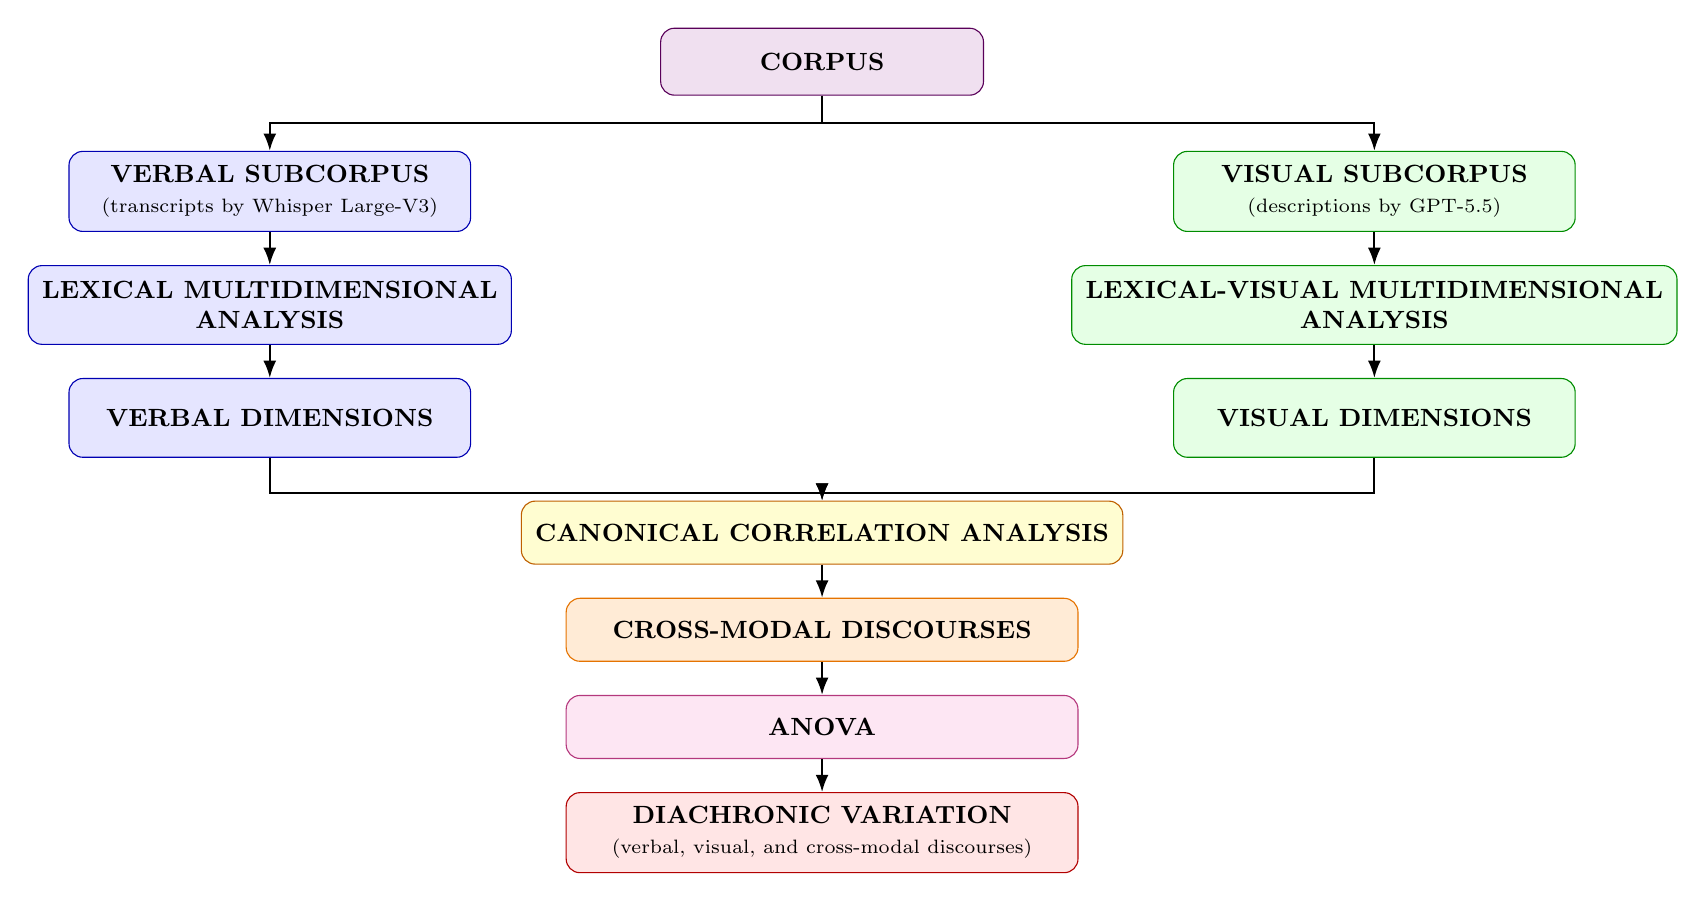
\begin{tikzpicture}[
    font=\sffamily,
    node distance=0.42cm and 2.8cm,
    arrow/.style={
        -{Latex[length=2.2mm]},
        thick,
        draw=black
    },
    corpus/.style={
        draw=violet!70!black,
        fill=violet!12,
        rounded corners=5pt,
        align=center,
        minimum width=4.1cm,
        minimum height=0.85cm,
        inner sep=5pt,
        font=\bfseries\small
    },
    verbal/.style={
        draw=blue!70!black,
        fill=blue!10,
        rounded corners=5pt,
        align=center,
        minimum width=5.1cm,
        minimum height=1cm,
        inner sep=5pt,
        font=\small
    },
    visual/.style={
        draw=green!55!black,
        fill=green!10,
        rounded corners=5pt,
        align=center,
        minimum width=5.1cm,
        minimum height=1cm,
        inner sep=5pt,
        font=\small
    },
    cca/.style={
        draw=orange!75!black,
        fill=yellow!18,
        rounded corners=5pt,
        align=center,
        minimum width=6.5cm,
        minimum height=0.8cm,
        inner sep=5pt,
        font=\bfseries\small
    },
    crossmodal/.style={
        draw=orange!90!black,
        fill=orange!16,
        rounded corners=5pt,
        align=center,
        minimum width=6.5cm,
        minimum height=0.8cm,
        inner sep=5pt,
        font=\bfseries\small
    },
    anova/.style={
        draw=magenta!70!black,
        fill=magenta!10,
        rounded corners=5pt,
        align=center,
        minimum width=6.5cm,
        minimum height=0.8cm,
        inner sep=5pt,
        font=\bfseries\small
    },
    diachronic/.style={
        draw=red!70!black,
        fill=red!10,
        rounded corners=5pt,
        align=center,
        minimum width=6.5cm,
        minimum height=1cm,
        inner sep=5pt,
        font=\small
    }
]

% Corpus
\node[corpus] (corpus)
{\textbf{CORPUS}};

% Subcorpora
\node[verbal, below left=0.7cm and 2.4cm of corpus] (verbal)
{\textbf{VERBAL SUBCORPUS}\\
\scriptsize (transcripts by Whisper Large-V3)};

\node[visual, below right=0.7cm and 2.4cm of corpus] (visual)
{\textbf{VISUAL SUBCORPUS}\\
\scriptsize (descriptions by GPT-5.5)};

% Analyses
\node[verbal, below=of verbal] (lexical)
{\textbf{LEXICAL MULTIDIMENSIONAL}\\
\textbf{ANALYSIS}};

\node[visual, below=of visual] (lexicalvisual)
{\textbf{LEXICAL-VISUAL MULTIDIMENSIONAL}\\
\textbf{ANALYSIS}};

% Dimensions
\node[verbal, below=of lexical] (verbdim)
{\textbf{VERBAL DIMENSIONS}};

\node[visual, below=of lexicalvisual] (visdim)
{\textbf{VISUAL DIMENSIONS}};

% Canonical correlation
\node[cca, below=1.05cm of $(verbdim)!0.5!(visdim)$] (cca)
{\textbf{CANONICAL CORRELATION ANALYSIS}};

% Cross-modal
\node[crossmodal, below=of cca] (cross)
{\textbf{CROSS-MODAL DISCOURSES}};

% ANOVA
\node[anova, below=of cross] (anova)
{\textbf{ANOVA}};

% Diachronic variation
\node[diachronic, below=of anova] (dia)
{\textbf{DIACHRONIC VARIATION}\\
\scriptsize (verbal, visual, and cross-modal discourses)};

% Arrows from corpus
\draw[arrow]
(corpus.south) -- ++(0,-0.35) -| (verbal.north);

\draw[arrow]
(corpus.south) -- ++(0,-0.35) -| (visual.north);

% Verbal flow
\draw[arrow] (verbal) -- (lexical);
\draw[arrow] (lexical) -- (verbdim);

% Visual flow
\draw[arrow] (visual) -- (lexicalvisual);
\draw[arrow] (lexicalvisual) -- (visdim);

% Merge into CCA
\draw[arrow]
(verbdim.south) -- ++(0,-0.45)
-| (cca.north);

\draw[arrow]
(visdim.south) -- ++(0,-0.45)
-| (cca.north);

% Final sequence
\draw[arrow] (cca) -- (cross);
\draw[arrow] (cross) -- (anova);
\draw[arrow] (anova) -- (dia);

\end{tikzpicture}
}

\end{frame}
%===================================================

%===================================================
% Slide da DIMENSÃO
% ==================================================
%\begin{frame}{Multi-Dimensional Perspective}
%\begin{columns}[onlytextwidth]
%  % -------- LEFT: table --------
%  \begin{column}{0.55\textwidth}
%    \small
%    \centering
%    \begin{tabular}{rlll}
%    \toprule
%    Dimensions & Poles \\
%    \midrule
%    1 & Pos. & Positive Dimension 1 \\
%      & Neg. & Negative Dimension 1 \\
%    2 & Pos. & Positive Dimension 2 \\
%      & Neg. & Negative Dimension 2 \\
%    3 & Pos. & Positive Dimension  $n$\\
%      & Neg. & Negative Dimension $n$ \\
%    \bottomrule
%    \end{tabular}
%
%\vspace{2em}
%%---------------------Texts Distributed-------------------------------
%  \begin{tikzpicture}
%    %blocks
%    \tikzstyle{block} = [rectangle, rounded corners, text=black, text centered, draw=black,
%                         font=\footnotesize, text width=1in, minimum height=.25in]
%   \tikzstyle{line}  = [>=latex,<->,draw=black,line width=1pt]
%    \node[block,fill=green!70,text=black] (subj) at (-1.5,-1.5) {+Positive Pole};
%    \node[block,fill=red!70,text=white]   (obj)  at ( 3.5,-1.5)  {--Negative Pole};
%
%     %arrow
%    \draw[line] (subj) to[in=180,out=0] (obj);
%     %---- BRACE (standard, not flattened) ----
%     %Place it close to the arrow (small raise), make it thinner, and lift the label.
%    \draw[
%      black,
%      line width=0.8pt,
%      decorate,
%      decoration={brace, amplitude=14pt, raise=.1pt}
%    ]
%      ($(subj.north east)!0.05!(obj.north west)$)
%        -- ($(obj.north west)!0.05!(subj.north east)$)
%      node[midway, yshift=25pt, text=black]{Texts Distributed};
%  \end{tikzpicture}
%
%  \end{column}
%
%\end{columns}
%
%\end{frame}
%===================================================

\begin{frame}{Multi-Dimensional Perspective}
\begin{columns}[onlytextwidth]
  % -------- LEFT: table --------
  \begin{column}{0.55\textwidth}
    \small
    \centering
    \begin{tabular}{rll}
    \toprule
    Dim. & Pole & Poles \\
    \midrule
    1 & Pos. & Positive Dimension 1 \\
      & Neg. & Negative Dimension 1 \\
    2 & Pos. & Positive Dimension 2 \\
      & Neg. & Negative Dimension 2 \\
    3 & Pos. &Positive Dimension  $n$\\
      & Neg. & Negative Dimension $n$ \\
      \bottomrule
    \end{tabular}

\vspace{2em}

  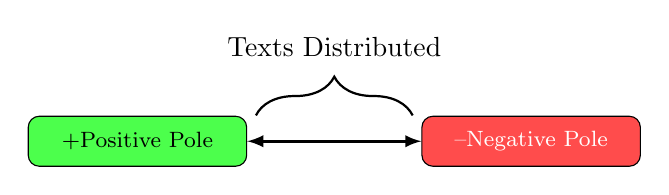
\begin{tikzpicture}
    % blocks
    \tikzstyle{block} = [rectangle, rounded corners, text=black, text centered, draw=black,
                         font=\footnotesize, text width=1in, minimum height=.25in]
   \tikzstyle{line}  = [>=latex,<->,draw=black,line width=1pt]
    \node[block,fill=green!70,text=black] (subj) at (-1.5,-1.5) {+Positive Pole};
    \node[block,fill=red!70,text=white]   (obj)  at ( 3.5,-1.5)  {--Negative Pole};
    % arrow
    \draw[line] (subj) to[in=180,out=0] (obj);
    % ---- BRACE (standard, not flattened) ----
    % Place it close to the arrow (small raise), make it thinner, and lift the label.
    \draw[
      black,
      line width=0.8pt,
      decorate,
      decoration={brace, amplitude=14pt, raise=.1pt}
    ]
      ($(subj.north east)!0.05!(obj.north west)$)
        -- ($(obj.north west)!0.05!(subj.north east)$)
      node[midway, yshift=25pt, text=black]{Texts Distributed};
  \end{tikzpicture}

  \end{column}

  % -------- RIGHT: tikz --------
  \vspace{1em}
  \begin{column}{0.45\textwidth}
    \centering
    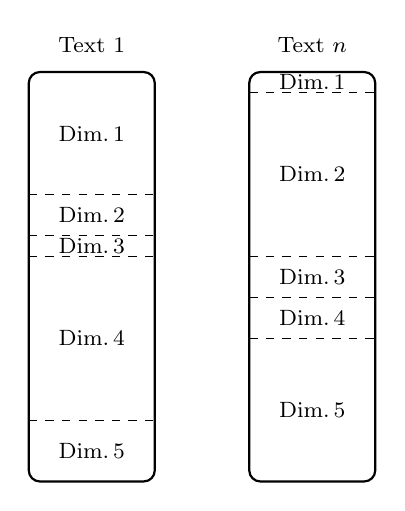
\begin{tikzpicture}
      % simple knobs (shrink a bit to fit side-by-side)
      \def\W{1.6cm}    % block width
      \def\H{5.2cm}    % block height
      \def\Gap{1.2cm}  % horizontal gap

      % ===================== LEFT BLOCK =====================
      % order top→bottom: 30%, 10%, 5%, 40%, 15%
      \begin{scope}[shift={(0,0)}]
        % outline
        \draw[rounded corners, thick] (0,0) rectangle (\W,\H);

        % dashed separators measured from bottom, but placed to keep Dim.1 at TOP
        \pgfmathsetlengthmacro{\yLone}{0.70*\H}  % top 30% ends at 70%
        \pgfmathsetlengthmacro{\yLtwo}{0.60*\H}  % then 10%
        \pgfmathsetlengthmacro{\yLthr}{0.55*\H}  % then 5%
        \pgfmathsetlengthmacro{\yLfour}{0.15*\H} % then 40%, leaving bottom 15%
        \draw[dashed] (0,\yLone) -- (\W,\yLone);
        \draw[dashed] (0,\yLtwo) -- (\W,\yLtwo);
        \draw[dashed] (0,\yLthr) -- (\W,\yLthr);
        \draw[dashed] (0,\yLfour) -- (\W,\yLfour);

        % title
        \node[font=\footnotesize] at (.5*\W, \H + .35cm) {Text 1};

        % segment labels centered in each band (top→bottom)
        \node[font=\footnotesize] at (.5*\W, 0.85*\H)  {Dim.\,1};   % (1 + .70)/2
        \node[font=\footnotesize] at (.5*\W, 0.65*\H)  {Dim.\,2};   % (.70 + .60)/2
        \node[font=\footnotesize] at (.5*\W, 0.575*\H) {Dim.\,3};   % (.60 + .55)/2
        \node[font=\footnotesize] at (.5*\W, 0.35*\H)  {Dim.\,4};   % (.55 + .15)/2
        \node[font=\footnotesize] at (.5*\W, 0.075*\H) {Dim.\,5};   % (.15 + 0)/2
      \end{scope}

      % ===================== RIGHT BLOCK =====================
      % order top→bottom: 5%, 40%, 10%, 10%, 35%
      \begin{scope}[shift={(\W+\Gap,0)}]
        % outline
        \draw[rounded corners, thick] (0,0) rectangle (\W,\H);

        % dashed separators for top→bottom ordering
        \pgfmathsetlengthmacro{\yRone}{0.95*\H} % top 5% ends at 95%
        \pgfmathsetlengthmacro{\yRtwo}{0.55*\H} % then 40%
        \pgfmathsetlengthmacro{\yRthr}{0.45*\H} % then 10%
        \pgfmathsetlengthmacro{\yRfour}{0.35*\H}% then 10%, leaving bottom 35%
        \draw[dashed] (0,\yRone) -- (\W,\yRone);
        \draw[dashed] (0,\yRtwo) -- (\W,\yRtwo);
        \draw[dashed] (0,\yRthr) -- (\W,\yRthr);
        \draw[dashed] (0,\yRfour) -- (\W,\yRfour);

        % title
        \node[font=\footnotesize] at (.5*\W, \H + .35cm) {Text $n$};

        % segment labels centered in each band (top→bottom)
        \node[font=\footnotesize] at (.5*\W, 0.975*\H) {Dim.\,1};  % (1 + .95)/2
        \node[font=\footnotesize] at (.5*\W, 0.75*\H)  {Dim.\,2};  % (.95 + .55)/2
        \node[font=\footnotesize] at (.5*\W, 0.50*\H)  {Dim.\,3};  % (.55 + .45)/2
        \node[font=\footnotesize] at (.5*\W, 0.40*\H)  {Dim.\,4};  % (.45 + .35)/2
        \node[font=\footnotesize] at (.5*\W, 0.175*\H) {Dim.\,5};  % (.35 + 0)/2
      \end{scope}
    \end{tikzpicture}
  \end{column}
\end{columns}
\end{frame}



{
\setbeamercolor{background canvas}{bg=blue}
\begin{frame}[c,plain]{}
\Huge
\centering
  \textcolor{white}{Findings}
\end{frame}
}

\nologo
\section{Findings}
% tem que ter esse este espaço entre section name e begin frame
\begin{frame}{VERBAL DIMENSIONS - Lexical Multidimensional Analysis (LMDA)}
\footnotesize
\begin{itemize}
    \item \textbf{Pos. Dim. 1}: Modernization of Female Domesticity
    \item \textbf{Neg. Dim. 1}: Neoliberal Self-Management​
    \item \textbf{Pos. Dim. 2}: Market-Delivered Betterment​
    \item \textbf{Neg. Dim. 2}: Market-Enabled Responsibilized Self-Management
    \item \textbf{Pos. Dim. 3}: Consumer Modernity as Masculine Social Authority
    \item \textbf{Neg. Dim. 3}: Products as Memorable Experiences​
    \item \textbf{Pos. Dim. 4}: Market-Constructed Consumer Differentiation
    \item \textbf{Neg. Dim. 4}: The Expected Mid-Century Housewife Lifestyle
\end{itemize}
\end{frame}

%\begin{frame}{Lexical Multidimensional Analysis (LMDA)}
%\footnotesize
%\begin{itemize}
%    \item \textbf{Pos. Dim. 5}: Market-Mediated Incompleteness​
%    \item \textbf{Neg. Dim. 5}:  Competitive Innovation and Perpetual Consumer Dissatisfaction​
%    \item \textbf{Pos. Dim. 6}: Gentle domestic cleanliness and Beauty​
%   \item \textbf{Neg. Dim. 6}: Demonstrated product utility \& Everyday Convenience
%    \item \textbf{Pos. Dim. 7}: Product-mechanism demonstration
%    \item \textbf{Neg. Dim. 7}: Everyday care \& Reassurance discourse​
%    \item \textbf{Pos. Dim. 8}: Mid-century promotional sales-pitch discourse
%    \item \textbf{Neg. Dim. 8}: Product-detail, proof, and transaction discourse
% \end{itemize}
% \end{frame}

{
\setbeamercolor{background canvas}{bg=blue}
\begin{frame}[c,plain]{}
    \Huge
    \centering
    \textcolor{white}{Dimension 1}
\end{frame}
}

   
\begin{frame}{VERBAL POSITIVE DIMENSION 1: Modernization of Female Domesticity}
   \footnotesize
\begin{block}{Variables:}
   \small
remember (.74), wonderful (.73), (quality (.69)), kitchen (.67), (fact (.63)), little (.63), own (.63), much (.61), color (.58), show (.57), important (.54), (set (.54)), (fast (.53)), (fit (.53)), last (.53), easy (.49), (fresh (.49)), water (.49), \textcolor{red}{\textbf{girl (.48)}}, (beautiful (.47)), (bright (.47)), (fine (.47)), keep (.47), (safe (.47)), sure (.47), (automatic (.46)), friend (.46), light (.46), many (.46), other (.46), (famous (.45)), (rca (.45)), (buy (.44)), (amazing (.43)), (wash (.43)), (white (.43)), (course (.42)), (hear (.42)), look (.42), (product (.42)), (lovely (.41)), (mean (.41)), (picture (.41)), put (.41), know (.40), take (.40), (box (.39)), (dealer (.39)), right (.39), (victor (.39)), give (.38), see (.38), (extra (.37)), (tube (.37)), \textbf{(woman (.37))}, (bottle (.36)), (flavor (.36)), make (.36), (rich (.36)), (room (.36)), (special (.36)), come (.35), (detergent (.35)), (control (.34)), (exciting (.34)), (plenty (.34)), call (.33), (eat (.33)), (enjoy (.33)), thing (.32), (car (.31)), (example (.31)), (happen (.31)), (most (.30))
%\ldots
%\textcolor{red}{\textbf{Corpus}}
\end{block}
\end{frame}

%\begin{frame}{POSITIVE DIMENSION 1: Modernization of Female Domesticity}
   %\footnotesize
   %\begin{block}{Interpretation}
   %\small
%\begin{itemize}
%\item Discourse of household modernization through consumption.
%\item The recurrent combination of domestic vocabulary (kitchen, wash, water, detergent), technological references (automatic, control, RCA, Victor, set), and positive evaluative terms (quality, wonderful, safe, beautiful, fine) constructs consumer goods as instruments of progress within everyday life.
%\item Household activities are repeatedly represented as tasks that can be simplified, improved, or optimized through modern products and technologies.
%\item As a result, the dimension promotes a socially shared representation of the home as a space of continuous improvement achieved through consumption.
%\item From a sociocognitive perspective, the discourse reproduces a cultural framework in which modernity, convenience, and domestic well-being are closely associated with consumer goods.
%\end{itemize}
%\end{block}
%\end{frame}

\begin{frame}{VERBAL POSITIVE DIMENSION 1: Modernization of Female
Domesticity}
\begin{exampleblock}{Examples:}
\begin{itemize}
    \small
    \item "XXXXXX."
    \item "XXXXXX."
\end{itemize}
\end{exampleblock}
\end{frame}


\begin{frame}{VERBAL NEGATIVE DIMENSION 1: Neoliberal Self-Management}
   \footnotesize
\begin{block}{Variables:}
   \small
employee (-.88), current (-.77), nintendo (-.71), card (-.70), information (-.68), select (-.68), ai (-.65), bacon (-.64), deal (-.64), prescription (-.64), present (-.64), computer (-.63), wireless (-.63), team (-.62), search (-.61), technology (-.61), rock (-.59), join (-.55), kenner (-.55), (lease (-.54)), daily (-.52), holiday (-.51), (class (-.50)), unique (-.50), video (-.50), (hurry (-.48)), gas (-.42), support (-.42), toilet (-.41), johnson (-.40), network (-.40), nylon (-.40), (sink (-.34)), gotta (-.33), (length (-.31)), wrong (-.31)
%\ldots  
\end{block}   
\end{frame}

%\begin{frame}{NEGATIVE DIMENSION 1: Neoliberal Self-Management}
%   \footnotesize
%   \begin{block}{Interpretation:}
%   \small
%   \begin{itemize}
%\item Discourse is conveyed through references to technology, information systems, artificial intelligence, workplace services, and eligibility-based commercial offers.
%\item The loading words (employee, current, deal, lease, card, information, AI, technology, computer, wireless, team, support) point to commercials that emphasize technical innovation, service infrastructures, and specific conditions for accessing products or promotions.
%\item Advertised products are frequently presented as technological solutions, workplace tools, support services, or special offers available to particular groups of consumers. As such, the dimension constructs consumption through technology, information, and institutional credibility.
%\item The repeated presence of technical vocabulary, service-oriented claims, and eligibility conditions gives the discourse a strongly functional and transactional orientation. 
%\end{itemize}
%\end{block}
%   \end{frame}


\begin{frame}{VERBAL NEGATIVE DIMENSION 1: Neoliberal Self-Management}
    \small
\begin{exampleblock}{Examples:}
\begin{itemize}
    \item "Yet xxxxx."
    \item "But if xxxxx."   
\end{itemize}
\end{exampleblock}
\end{frame}


\begin{frame}{VISUAL DIMENSIONS - Lexical Multidimensional Analysis (LMDA)}
    \footnotesize
\begin{itemize}
    \item \textbf{Pos. Dim. 1}: The market structures how contemporary life is managed
    \item \textbf{Neg. Dim. 1}: Market-mediated female domesticity \& Male-structured visibility​
    \item \textbf{Pos. Dim. 2}: The naturalization of masculine mobility, agency \& control ​
    \item \textbf{Neg. Dim. 2}: Market-delivered betterment
    \item \textbf{Pos. Dim. 3}: Consumer technology as personal progress
    \item \textbf{Neg. Dim. 3}: ​
    \item \textbf{Pos. Dim. 4}: 
    \item \textbf{Neg. Dim. 4}: 
\end{itemize}
\end{frame}


\begin{frame}{VISUAL POSITIVE DIMENSION 1: }
   \footnotesize
\begin{block}{Variables:} arctic (-.87), republic (-.83), amazon (-.82)
\end{block}
\end{frame}


\begin{frame}{VISUAL POSITIVE DIMENSION 1: }
    \small
\begin{alertblock}{Examples:}
\begin{itemize}
    \item “XXXX.”
    \item “To address this XXXXXX.” 
\end{itemize}
\end{alertblock}
\end{frame}


\begin{frame}{CANONICAL ANALYSIS - AMD Lexical \& AMD Visual}
    \footnotesize
\begin{itemize}
    \item \textbf{DIM-L 1 (LEXICAL Dimension 1)}: 
    \item \textbf{DIM-V 4 (Visual Dimension 4)}: ​
    \vspace{1cm}
    \item xxxxxxx
\end{itemize}
\end{frame}


\begin{frame}{DIACHRONIC ANALYSIS}
    \footnotesize
\begin{itemize}
    \item xxxxx
    \vspace{1cm}
    \item xxxxxxx
\end{itemize}
\end{frame}


{
\setbeamercolor{background canvas}{bg=blue}
\begin{frame}[c,plain]{}
    \vspace*{1cm}
    \centering
    \Huge
    \textcolor{white}{Final Remarks}
\end{frame}
}


\section{Final Remarks}
% tem que ter esse este espaço entre section name e begin frame
\begin{frame}[allowframebreaks]{Final Remarks}
    \footnotesize
\begin{itemize}
    \item The findings suggest that human-authored and LLM-generated texts share many of the same environmental discourses, particularly those related to climate justice, environmental responsibility, corporate accountability, and climate action. However, they organise these discourses differently.
    \item LLMs can be understood as machines of abstraction. Because they are trained on vast quantities of texts produced from many different perspectives, they tend to compress this diversity into recurrent and averaged patterns.
    \item In this process, many concrete details are lost. What remains are broader categories, general concepts, and more abstract formulations.
    \item As a result, LLM-generated discourses tend to operate at a more abstract level than human-authored discourse.
\end{itemize}
\end{frame}

\section{Thank you all!}
% tem que ter esse este espaço entre section name e begin frame
\begin{frame}[plain]
    \centering
    \vfill
    {\Huge Thank you!} \\
    \vspace{1cm}
    {\Large \textit{acmsantos70@gmail.com.br}}
    \vfill
\end{frame}

\appendix

\begin{frame}[allowframebreaks]{References}
\small

\printbibliography

\end{frame}

\end{document}

